\part{ФОРМИРОВАНИЕ ШУМА}
    \section*{Описание процесса формирования шума}
        Интервал распределения шума задан как $ (-\Delta y; \Delta y) $, где коэффициент $\Delta y$ вычисляется по формуле:
        $$
            \Delta y = max(|y^{T}|) \cdot
            \begin{Bmatrix}
                0,05 \\
                0,1 \\
                0,2
            \end{Bmatrix}
            =
            \begin{Bmatrix}
                1.092 \\
                2.184 \\
                4.367
            \end{Bmatrix}
        $$

        После вычисления значений шума, необходимо добавить их к теоретическим значениям в интересующих нас точках для получения экспериментальных значений.

        Можно составить блок-схему процесса генерации экспериментальных значений.

        \begin{center}
            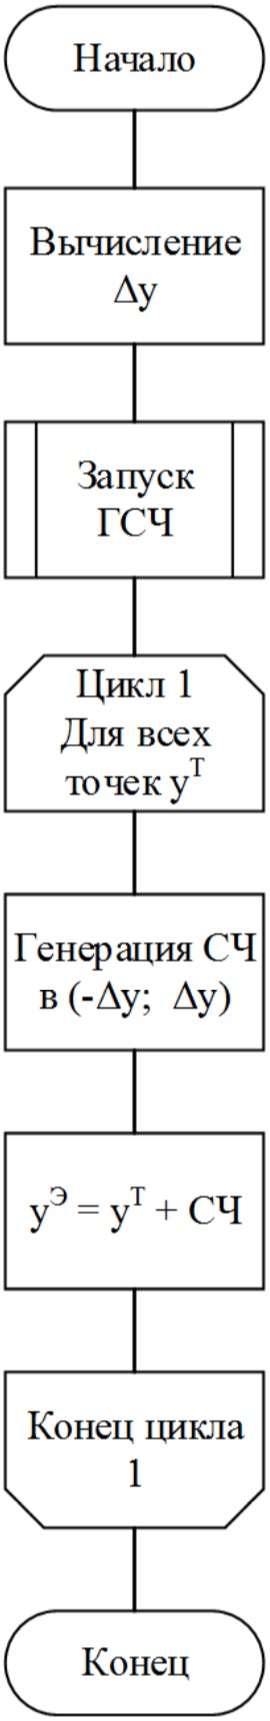
\includegraphics[scale=0.25]{img/block}
        \end{center}

    \section*{Проверка ГСЧ}
        \begin{center}
            \begin{tikzpicture}
                \begin{axis}[ybar, ymin=0, ymax=1200]
                    \addplot [fill, color=blue] table [col sep=comma] {data/precomputed/uniform-random.csv};
                    Гистограммы отражают исправную работу ГСЧ.
                \end{axis}
            \end{tikzpicture}
        \end{center}
        Гистограмма выше отражает факт равномерного распределения случайных чисел ГСЧ. Выбран интервал от $0$ до $1$, каждый столбец гистограмы -- интервал, равный $\dfrac{1}{10}$.

    \section*{Построим графики экспериментальных функций}
        \begin{center}
            \begin{tikzpicture}
                \begin{axis}[
                        width=17cm,
                        height=12cm,
                        xlabel=x,
                        ylabel=y,
                        minor tick num = 1,
                        grid = both,
                        legend style={at={(0.5,-0.1)},anchor=north}
                    ]
                    \addplot table [col sep=comma] {data/theor.csv};
                    \addlegendentry{$Y_{\text{теор.}}$}

                    \addplot table [col sep=comma] {data/exp1.csv};
                    \addlegendentry{$Y_{\text{Э}}(0.05)$}

                    \addplot table [col sep=comma] {data/exp2.csv};
                    \addlegendentry{$Y_{\text{Э}}(0.1)$}

                    \addplot table [col sep=comma] {data/exp3.csv};
                    \addlegendentry{$Y_{\text{Э}}(0.2)$}
                \end{axis}
            \end{tikzpicture}
        \end{center}
